%导数与函数极值

\pentry{导数\upref{Der}}
\begin{figure}[ht]
\vskip-10pt
\centering
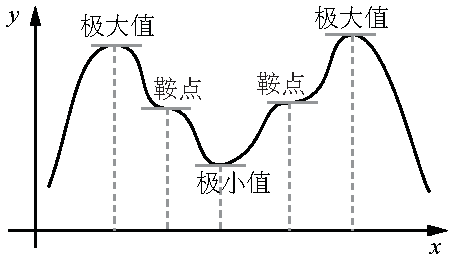
\includegraphics[width=0.75\textwidth]{./figures/DerMax.pdf}
\caption{导数为零的三种点} % 图太小!
\end{figure}

若一个一元函数 $y = f(x)$ 在考察的区间内处处可导(即对区间内的任何 $x$ 导数 $f'(x)$ 都存在),若某些 ${x_i}$ 能使 $f'(x_i) = 0$, 则在这些点处函数曲线的斜率为零.

而从函数图像来看,这样的点又分为三类: \textbf{极大值},\textbf{极小值},\textbf{鞍点}.

\begin{exam}{}
抛物线的极值点?%未完成

$x+1/x$ 的极值点?等等%未完成
\end{exam}













